% Options for packages loaded elsewhere
\PassOptionsToPackage{unicode}{hyperref}
\PassOptionsToPackage{hyphens}{url}
\PassOptionsToPackage{dvipsnames,svgnames,x11names}{xcolor}
%
\documentclass[
  letterpaper,
  DIV=11,
  numbers=noendperiod]{scrartcl}

\usepackage{amsmath,amssymb}
\usepackage{iftex}
\ifPDFTeX
  \usepackage[T1]{fontenc}
  \usepackage[utf8]{inputenc}
  \usepackage{textcomp} % provide euro and other symbols
\else % if luatex or xetex
  \usepackage{unicode-math}
  \defaultfontfeatures{Scale=MatchLowercase}
  \defaultfontfeatures[\rmfamily]{Ligatures=TeX,Scale=1}
\fi
\usepackage{lmodern}
\ifPDFTeX\else  
    % xetex/luatex font selection
\fi
% Use upquote if available, for straight quotes in verbatim environments
\IfFileExists{upquote.sty}{\usepackage{upquote}}{}
\IfFileExists{microtype.sty}{% use microtype if available
  \usepackage[]{microtype}
  \UseMicrotypeSet[protrusion]{basicmath} % disable protrusion for tt fonts
}{}
\makeatletter
\@ifundefined{KOMAClassName}{% if non-KOMA class
  \IfFileExists{parskip.sty}{%
    \usepackage{parskip}
  }{% else
    \setlength{\parindent}{0pt}
    \setlength{\parskip}{6pt plus 2pt minus 1pt}}
}{% if KOMA class
  \KOMAoptions{parskip=half}}
\makeatother
\usepackage{xcolor}
\setlength{\emergencystretch}{3em} % prevent overfull lines
\setcounter{secnumdepth}{5}
% Make \paragraph and \subparagraph free-standing
\makeatletter
\ifx\paragraph\undefined\else
  \let\oldparagraph\paragraph
  \renewcommand{\paragraph}{
    \@ifstar
      \xxxParagraphStar
      \xxxParagraphNoStar
  }
  \newcommand{\xxxParagraphStar}[1]{\oldparagraph*{#1}\mbox{}}
  \newcommand{\xxxParagraphNoStar}[1]{\oldparagraph{#1}\mbox{}}
\fi
\ifx\subparagraph\undefined\else
  \let\oldsubparagraph\subparagraph
  \renewcommand{\subparagraph}{
    \@ifstar
      \xxxSubParagraphStar
      \xxxSubParagraphNoStar
  }
  \newcommand{\xxxSubParagraphStar}[1]{\oldsubparagraph*{#1}\mbox{}}
  \newcommand{\xxxSubParagraphNoStar}[1]{\oldsubparagraph{#1}\mbox{}}
\fi
\makeatother


\providecommand{\tightlist}{%
  \setlength{\itemsep}{0pt}\setlength{\parskip}{0pt}}\usepackage{longtable,booktabs,array}
\usepackage{calc} % for calculating minipage widths
% Correct order of tables after \paragraph or \subparagraph
\usepackage{etoolbox}
\makeatletter
\patchcmd\longtable{\par}{\if@noskipsec\mbox{}\fi\par}{}{}
\makeatother
% Allow footnotes in longtable head/foot
\IfFileExists{footnotehyper.sty}{\usepackage{footnotehyper}}{\usepackage{footnote}}
\makesavenoteenv{longtable}
\usepackage{graphicx}
\makeatletter
\newsavebox\pandoc@box
\newcommand*\pandocbounded[1]{% scales image to fit in text height/width
  \sbox\pandoc@box{#1}%
  \Gscale@div\@tempa{\textheight}{\dimexpr\ht\pandoc@box+\dp\pandoc@box\relax}%
  \Gscale@div\@tempb{\linewidth}{\wd\pandoc@box}%
  \ifdim\@tempb\p@<\@tempa\p@\let\@tempa\@tempb\fi% select the smaller of both
  \ifdim\@tempa\p@<\p@\scalebox{\@tempa}{\usebox\pandoc@box}%
  \else\usebox{\pandoc@box}%
  \fi%
}
% Set default figure placement to htbp
\def\fps@figure{htbp}
\makeatother
% definitions for citeproc citations
\NewDocumentCommand\citeproctext{}{}
\NewDocumentCommand\citeproc{mm}{%
  \begingroup\def\citeproctext{#2}\cite{#1}\endgroup}
\makeatletter
 % allow citations to break across lines
 \let\@cite@ofmt\@firstofone
 % avoid brackets around text for \cite:
 \def\@biblabel#1{}
 \def\@cite#1#2{{#1\if@tempswa , #2\fi}}
\makeatother
\newlength{\cslhangindent}
\setlength{\cslhangindent}{1.5em}
\newlength{\csllabelwidth}
\setlength{\csllabelwidth}{3em}
\newenvironment{CSLReferences}[2] % #1 hanging-indent, #2 entry-spacing
 {\begin{list}{}{%
  \setlength{\itemindent}{0pt}
  \setlength{\leftmargin}{0pt}
  \setlength{\parsep}{0pt}
  % turn on hanging indent if param 1 is 1
  \ifodd #1
   \setlength{\leftmargin}{\cslhangindent}
   \setlength{\itemindent}{-1\cslhangindent}
  \fi
  % set entry spacing
  \setlength{\itemsep}{#2\baselineskip}}}
 {\end{list}}
\usepackage{calc}
\newcommand{\CSLBlock}[1]{\hfill\break\parbox[t]{\linewidth}{\strut\ignorespaces#1\strut}}
\newcommand{\CSLLeftMargin}[1]{\parbox[t]{\csllabelwidth}{\strut#1\strut}}
\newcommand{\CSLRightInline}[1]{\parbox[t]{\linewidth - \csllabelwidth}{\strut#1\strut}}
\newcommand{\CSLIndent}[1]{\hspace{\cslhangindent}#1}

\KOMAoption{captions}{tableheading}
\makeatletter
\@ifpackageloaded{caption}{}{\usepackage{caption}}
\AtBeginDocument{%
\ifdefined\contentsname
  \renewcommand*\contentsname{Table of contents}
\else
  \newcommand\contentsname{Table of contents}
\fi
\ifdefined\listfigurename
  \renewcommand*\listfigurename{List of Figures}
\else
  \newcommand\listfigurename{List of Figures}
\fi
\ifdefined\listtablename
  \renewcommand*\listtablename{List of Tables}
\else
  \newcommand\listtablename{List of Tables}
\fi
\ifdefined\figurename
  \renewcommand*\figurename{Figure}
\else
  \newcommand\figurename{Figure}
\fi
\ifdefined\tablename
  \renewcommand*\tablename{Table}
\else
  \newcommand\tablename{Table}
\fi
}
\@ifpackageloaded{float}{}{\usepackage{float}}
\floatstyle{ruled}
\@ifundefined{c@chapter}{\newfloat{codelisting}{h}{lop}}{\newfloat{codelisting}{h}{lop}[chapter]}
\floatname{codelisting}{Listing}
\newcommand*\listoflistings{\listof{codelisting}{List of Listings}}
\makeatother
\makeatletter
\makeatother
\makeatletter
\@ifpackageloaded{caption}{}{\usepackage{caption}}
\@ifpackageloaded{subcaption}{}{\usepackage{subcaption}}
\makeatother

\usepackage{bookmark}

\IfFileExists{xurl.sty}{\usepackage{xurl}}{} % add URL line breaks if available
\urlstyle{same} % disable monospaced font for URLs
\hypersetup{
  pdftitle={Spatial distribution of Gracillaria vermiculophylla in French and Spanish estuaries using Unmaned Aerial Vehicule.},
  pdfauthor={Simon Oiry¹; Bede Ffinian Rowe Davies¹; Pierre Gernez¹; Laurent Barillé¹},
  pdfkeywords={Remote Sensing, Invasive species, Coastal
Ecosystems, Biodiversity},
  colorlinks=true,
  linkcolor={blue},
  filecolor={Maroon},
  citecolor={Blue},
  urlcolor={Blue},
  pdfcreator={LaTeX via pandoc}}


\title{Spatial distribution of \emph{Gracillaria vermiculophylla} in
French and Spanish estuaries using Unmaned Aerial Vehicule.}
\author{Simon Oiry¹ \and Bede Ffinian Rowe Davies¹ \and Pierre
Gernez¹ \and Laurent Barillé¹}
\date{2024-12-13}

\begin{document}
\maketitle
\begin{abstract}
To be Written
\end{abstract}


\footnote{Institut des Substances et Organismes de la Mer, ISOMer,
  Nantes Université, UR 2160, F-44000 Nantes, France}

\section{Introduction}\label{introduction}

The introduction of Non-Indigenous Species (NIS) in terrestrial,
freshwater, and marine ecosystems is one of the major threats to
biodiversity worldwide. In particular, the proliferation and rapid
spread of Invasive Alien Species (IAS) can radically change the
structure and functioning of marine ecosystems, , requiring effective
inventorying and monitoring programs (Massé et al., 2023). In Europe,
874 NIS have been introduced to the marine environment so far
(i.e.~until 2020) and it is expected that the rate of biological
invasions will continue to increase in the coming years (Zenetos et al.,
2022). Macroalgae represent more than 40 \% of the NIS introduced to
Europe waters, with many species native to the Temperate Northern
Pacific (Williams and Smith, 2007). Amongst all invasive macroalgae,
\emph{Gracilaria vermiculophylla} (Papenfuss, 1967) (original name
\emph{Gracilariopsis vermiculophylla} (OHMI, 1956); also known as
\emph{Agarophyton vermiculophyllum} (Gurgel et al., 2018)), has spread
extensively from its native distribution range in Japan and Korea
(Terada and Yamamoto, 2002) across temperate estuaries in North America,
Europe, and other regions, facilitated by aquaculture and maritime
activities (Krueger-Hadfield et al., 2017; Rueness, 2005; Weinberger et
al., 2008). While \emph{G. vermiculophylla} can provide some ecosystem
services, such as habitat for invertebrates and juvenile fish (Davoult
et al., 2017), it often outcompetes native vegetation, alters sediment
composition (Nyberg et al., 2009), and disrupts trophic interactions
(Ginneken et al., 2018). In regions like the Baltic Sea and the eastern
United States, it has been documented to negatively affect native
fucoids and seagrasses (Firth et al., 2024; Thomsen et al., 2013; Van
Katwijk, 2003). These impacts underscore the importance of monitoring
and managing the spread of \emph{G. vermiculophylla}, particularly as
climate change and anthropogenic pressures continue to facilitate
biological invasions. \emph{G. vermiculophylla} success as an invader
stems from its tolerance to a wide range of environmental conditions,
including temperature (Sotka et al., 2018), nutrient variability (Abreu
et al., 2011) and salinity (Weinberger et al., 2008). Its growth
capacity at low salinities (Nyberg, 2007; Rueness, 2005) explains its
presence in the brackish waters of the Baltic Sea (Weinberger et al.,
2008) but also in the mesohaline sheltered part of estuaries of the
Atlantic coast of Europe \textbf{(Surget et al., 2017)}. It is also
present in confined areas of lagoons characterized by low hydrodynamism
(Abreu et al., 2011; Sfriso et al., 2012). In Europe, it was first
observed in 1996 in the Belon estuary (France) and later in many other
estuaries on the Brittany coast of France (Rueness, 2005). It can be
found on hard substrates such as invertebrate's tubes and shells
providing a substratum (Thomsen et al., 2007) or attached to pebbles and
rocks (Terada and Yamamoto, 2002) but the largest populations are
colonizing soft-bottom sediment and particularly estuarine intertidal
mudflats \textbf{(Surget et al., 2017)}. In this habitat, extensive dark
red mats are observed at low tide, covering vast areas that have largely
been unquantified in most studies. Therefore, \emph{G. vermiculophylla}
is capable of establishing populations in soft-bottom sediment habitats
that were previously devoid of macroalgae (Ramus et al., 2017). These
mats are usually monospecific with the alga thalli partially buried into
the mud (Rueness, 2005; Surget, 2017). Intertidal mats can however be
temporarily overgrown by ephemeral green macroalgae (Weinberger et al.,
2008). In the estuaries where \emph{G. vermiculophylla} was first
documented, large monospecific mats were reported to be confined to the
upper intertidal zones (Rueness, 2005); however, their spatial
distribution relative to the mudflat topography had not been
quantitatively assessed. In fact, \emph{G. vermiculophylla} has never
been mapped using remote sensing techniques, and existing descriptions
of its distribution lack spatially explicit mapping (Abreu et al., 2011;
Sfriso et al., 2012; Thomsen et al., 2007; Weinberger et al., 2008)

Remote sensing has revolutionized our ability to monitor and manage
coastal ecosystems, offering efficient and scalable methods for
detecting environmental changes in intertidal vegetation across a wide
range of spatio-temporal scales (Calleja et al., 2017; Davies et al.,
2024a, 2024b; Valle et al., 2015; Zoffoli et al., 2021). Among
remote-sensing technologies, drone-based imagery has recently emerged as
a particularly promising tool for studying the spatial distribution of
intertidal primary producers such as benthic microalgae (Román et al.,
2024, 2021), seagrass (Chand and Bollard, 2021; Duffy et al., 2018;
Román et al., 2021) and macroalgae (Diruit et al., 2022; Peidro-Devesa
et al., 2024). While it lacks the temporal consistency of satellite
missions, drone remote sensing makes it possible to acquire at extremely
high spatial resolution (i.e.~cm-scale), rapidly target specific areas
of interest, and to provide observations in overcast conditions. In
particular, the potential of drone remote sensing for monitoring the
surface area occupied by IAS has been demonstrated (Roca et al., 2022).
Drone-based photogrammetry also makes it possible to characterize the
distribution of intertidal vegetation together with mudflat
geomorphology, thus improving our understanding of primary producers
patterning (Brunier et al., 2022; Douglas et al., 2024).

In this study, a drone-based multispectral remote sensing approach was
applied to map \emph{G. vermiculophylla} spatial distribution at a
very-high spatial resolution in three intertidal estuaries of European
Atlantic coast. We adapted the neural network classification model
DISCOV (Drone Intertidal Substrate Classification Of Vegetation, Oiry et
al. (2024b), Oiry et al. (2024a)) by specifically training the model
with a new class corresponding to \emph{G. vermiculophylla}. A
validation dataset was obtained from \emph{in situ} data to estimate the
classification accuracy. LIDAR data were concurrently acquired to
accurately map the intertidal elevation. We used a Generalized Additive
Model (GAM) to examine the relationship between the seaweed spatial
distribution and spatial metrics quantifying the mudflat topography. We
expected the presence of G. vermiculophylla in mudflats to be associated
to a specific height range as well as being more closely related to flat
areas of the intertidal zone.

\section{Materiel \& Methods}\label{materiel-methods}

\subsection{Study sites}\label{study-sites}

Field campaigns were conducted at three study sites in France and Spain.
At each site, two locations were investigated
Figure~\ref{fig-location_sites}. The Aven \& Belon Estuary in South
Brittany, France (Figure~\ref{fig-location_sites} A \& C), is a dynamic
ria-type system hosting diverse habitats, including sandy tidal flats
and subtidal zones with coarse, marine-origin sediments (Castaing and
Guilcher, 1995; Michel et al., 2021). These habitats support key benthic
species such as \emph{Scrobicularia plana}, \emph{Cerastoderma edule},
and \emph{Tellina tenuis}, which play essential roles in sediment
bioturbation and nutrient cycling (Blanchet et al., 2014; Tankoua et
al., 2011). The estuary serves as a nursery for juvenile fish and a
feeding ground for migratory birds, with its ecological productivity
driven by a mix of euryhaline and marine species adapted to salinity
gradients (Blanchet et al., 2014). Oyster farming, particularly
\emph{Crassostrea gigas}, is a dominant activity, altering sediment
dynamics and local biodiversity (Michel et al., 2021). Despite its
ecological richness, the estuary faces pressures from nutrient loading
and physical alterations, with bioindicators like \emph{S. plana} used
to monitor the impacts of salinity, sediment quality, and pollution
(Tankoua et al., 2011).

The Saja-Besaya Estuary, situated along the Cantabrian Sea in northern
Spain, is characterized by the confluence of the Saja and Besaya rivers
near Torrelavega (Figure~\ref{fig-location_sites} C). The estuary, also
known as San Martín de la Arena or Suances Estuary, has been subject to
significant anthropogenic pressures, including industrial developments
throughout the 20th century. These activities have led to contamination
from mining, paper manufacturing, and carbonate discharges, classifying
the estuary as highly polluted near its upper reaches (Ortega et al.,
2005). This contamination impacts the estuarine ecosystem, including
water quality and biodiversity, with minimal aquatic life and sparse
riverbank vegetation in its lower sections (Romero et al., 2008).

\phantomsection\label{cell-fig-location_sites}
\begin{figure}[H]

\centering{

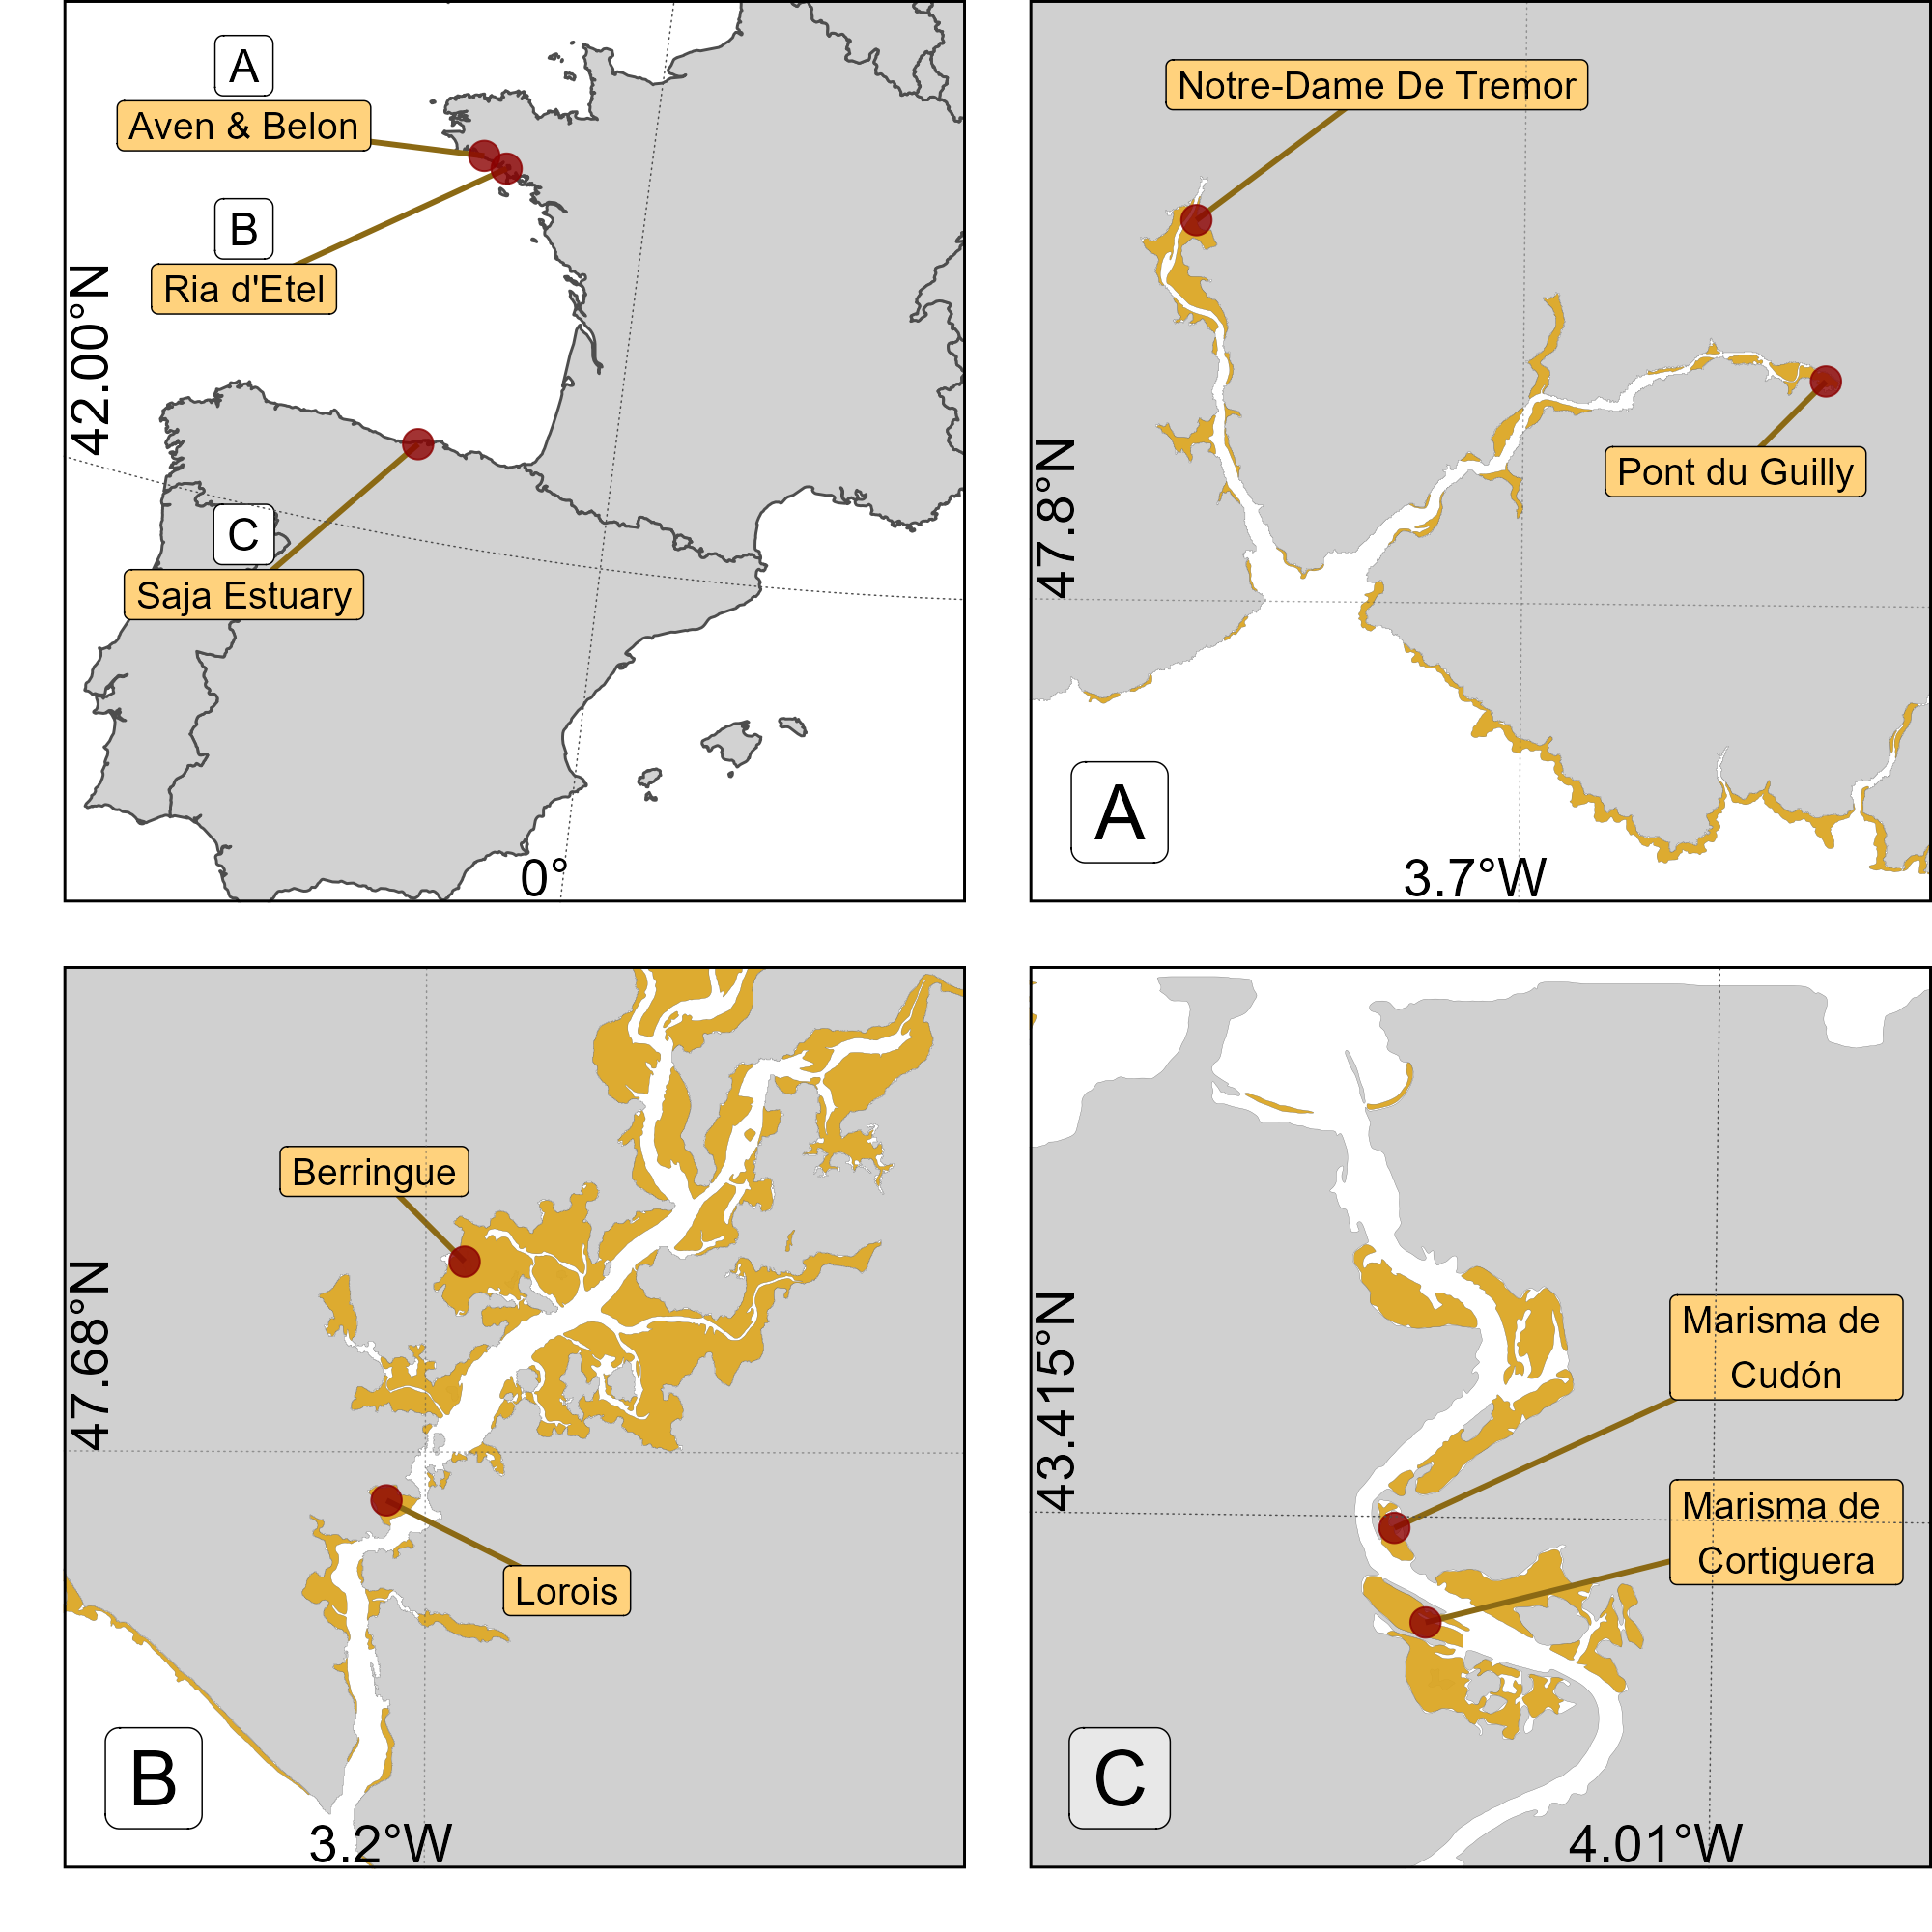
\includegraphics[width=0.95\linewidth,height=\textheight,keepaspectratio]{Figures/Low_res/Figure1/Map_site.png}

}

\caption{\label{fig-location_sites}Location of the drone flights. A:
Flights made in Aven Estuary, France; B: Flights made in Bélon Estuary,
France; C: Flights made in Saja Estuaries, Spain. Golden polygons
represent intertidal areas.}

\end{figure}%

\subsection{Remote sensing data acquisition and
pre-processing}\label{sec-DroneFlights}

\begin{table}

\caption{\label{tbl-flights}List of drone flights, summarising the
location, the date, and the total extent of each flight (in hectars).}

\centering{


\includegraphics[width=8.84in,height=\textheight,keepaspectratio]{Figures/High_res/table_flights.png}

}

\end{table}%

A total of 6 drone flights were done spread in the 3 study sites. Each
time, flights were done at an altitude of 120 m and at a speed of 10
m.s\textsuperscript{-1} (Table~\ref{tbl-flights}).

\subsubsection{Multispectral data}\label{sec-photo}

At each location, reflectance images with a resolution of 1.2 million
pixels were captured using a DJI Matrice 300 quadcopter drone equipped
with a Micasense RedEdge Dual MX multispectral camera. The camera
recorded data across ten spectral bands, spanning from blue to
near-infrared (NIR) wavelengths (444, 475, 531, 560, 650, 668, 705, 717,
740, and 840 nm) (). To ensure consistent lighting conditions, the
drone's flight trajectory was aligned to maintain a solar azimuth angle
of 90 degrees. Image acquisition was carried out with an overlap of 70\%
between side-by-side images and 80\% between successive images along the
flight path. A downwelling light sensor (DLS2) was used to measure
real-time irradiance, enabling the correction of reflectance values for
variations in light intensity caused by cloud cover during the flight.
The raw image data were subsequently calibrated to reflectance using a
calibration panel with \textasciitilde50\% reflectivity, provided by the
camera's manufacturer. Images were processed using structure-from-motion
photogrammetry software (Agisoft, 2019) to generate multispectral
ortho-mosaics for each flight. The ortho-mosaicking workflow was
consistent across all flights. Initially, key tie points were identified
within each image and across overlapping images to create a sparse point
cloud. This point cloud was refined by removing noisy points using a
reprojection accuracy metric. Subsequently, a dense point cloud was
generated using a structure-from-motion algorithm. A digital surface
model (DSM) was then created through surface interpolation of the dense
point cloud, which served as the basis for reconstructing the
multispectral ortho-image (Nebel et al., 2020). The resolution of the
multispectral ortho-mosaic obtained were 8 cm per pixel.

\subsubsection{LiDAR data}\label{lidar-data}

LiDAR standing for Light Detection and Ranging uses lasers to measure
distances by timing reflected pulses, creating detailed 3D maps of
surfaces.

Using the Matrice 300 Series Dual Gimbal Connector, a DJI Zenmuse L1
LiDAR and RGB sensor was mounted on the drone alongside a multispectral
camera. This setup enabled the simultaneous capture of LiDAR point
clouds, high-resolution RGB images, and multispectral images collected
by the MicaSense RedEdge Dual MX during the same flight. The same
processing workflow as Section~\ref{sec-photo} was applied to process
LiDAR RGB images, resulting in ortho-mosaic with a resolution of 2.5 cm
per pixel. Since the mapping focused solely on flat surfaces without
dense vegetation, the LiDAR measured only a single return. Operating in
repetitive scanning mode with a sampling rate of 240 kHz, the system
achieved a point density of 350 points per square meter. The LiDAR point
cloud was extracted and converted into LAS format using DJI Terra
software. The LAS point cloud was then imported into Agisoft Metashape
(Agisoft, 2019) to generate a DEM with a resolution of 2.5 cm.

\subsection{Scene classification}\label{scene-classification}

A neural network classification model (DISCOV; Oiry et al. (2024b); Oiry
et al. (2024a)), previously applied with success to Micasense
reflectance data for mapping intertidal vegetation along the Portuguese
and French Atlantic coasts, has been used in this study. The training
dataset of DISCOV v1.0 has been updated. As shown by Oiry et al. (2024b)
the DISCOV v1.0 model (Oiry et al., 2024a) was trained using only 5771
Rhodophyceae pixel (3\% of the training dataset). To fill this gap the
original training dataset of DISCOV v1.0 was updated using new training
pixel coming from the 5 drone flights (Section~\ref{sec-DroneFlights}).

\section{Results}\label{results}

\subsection{Historical records in the Belon
estuary}\label{historical-records-in-the-belon-estuary}

A clear shift in sediment coloration over the paste 70 years were
observed, closely aligned with the subsequent proliferation of the
invasive red macroalga \emph{Gracilaria vermiculophylla}
(Figure~\ref{fig-HistoricalMap}). Before 1976, the sediments appeared
relatively light, indicating no detectable presence of this species.
Following its initial appearance in 1976, subtle darkening of the
sediment became discernible, coinciding with the early establishment of
\emph{G. vermiculophylla}. During the subsequent decades, the late 1970s
through the 1990s, this darkening trend became more pronounced and
widespread, reflecting an increasing spatial coverage and biomass of the
algae. By the early 2000s, and especially by 2024, the sediment
exhibited consistently darker tones, indicative of extensive and
persistent colonization by \emph{G. vermiculophylla}.

\phantomsection\label{cell-fig-HistoricalMap}
\begin{figure}[H]

\centering{

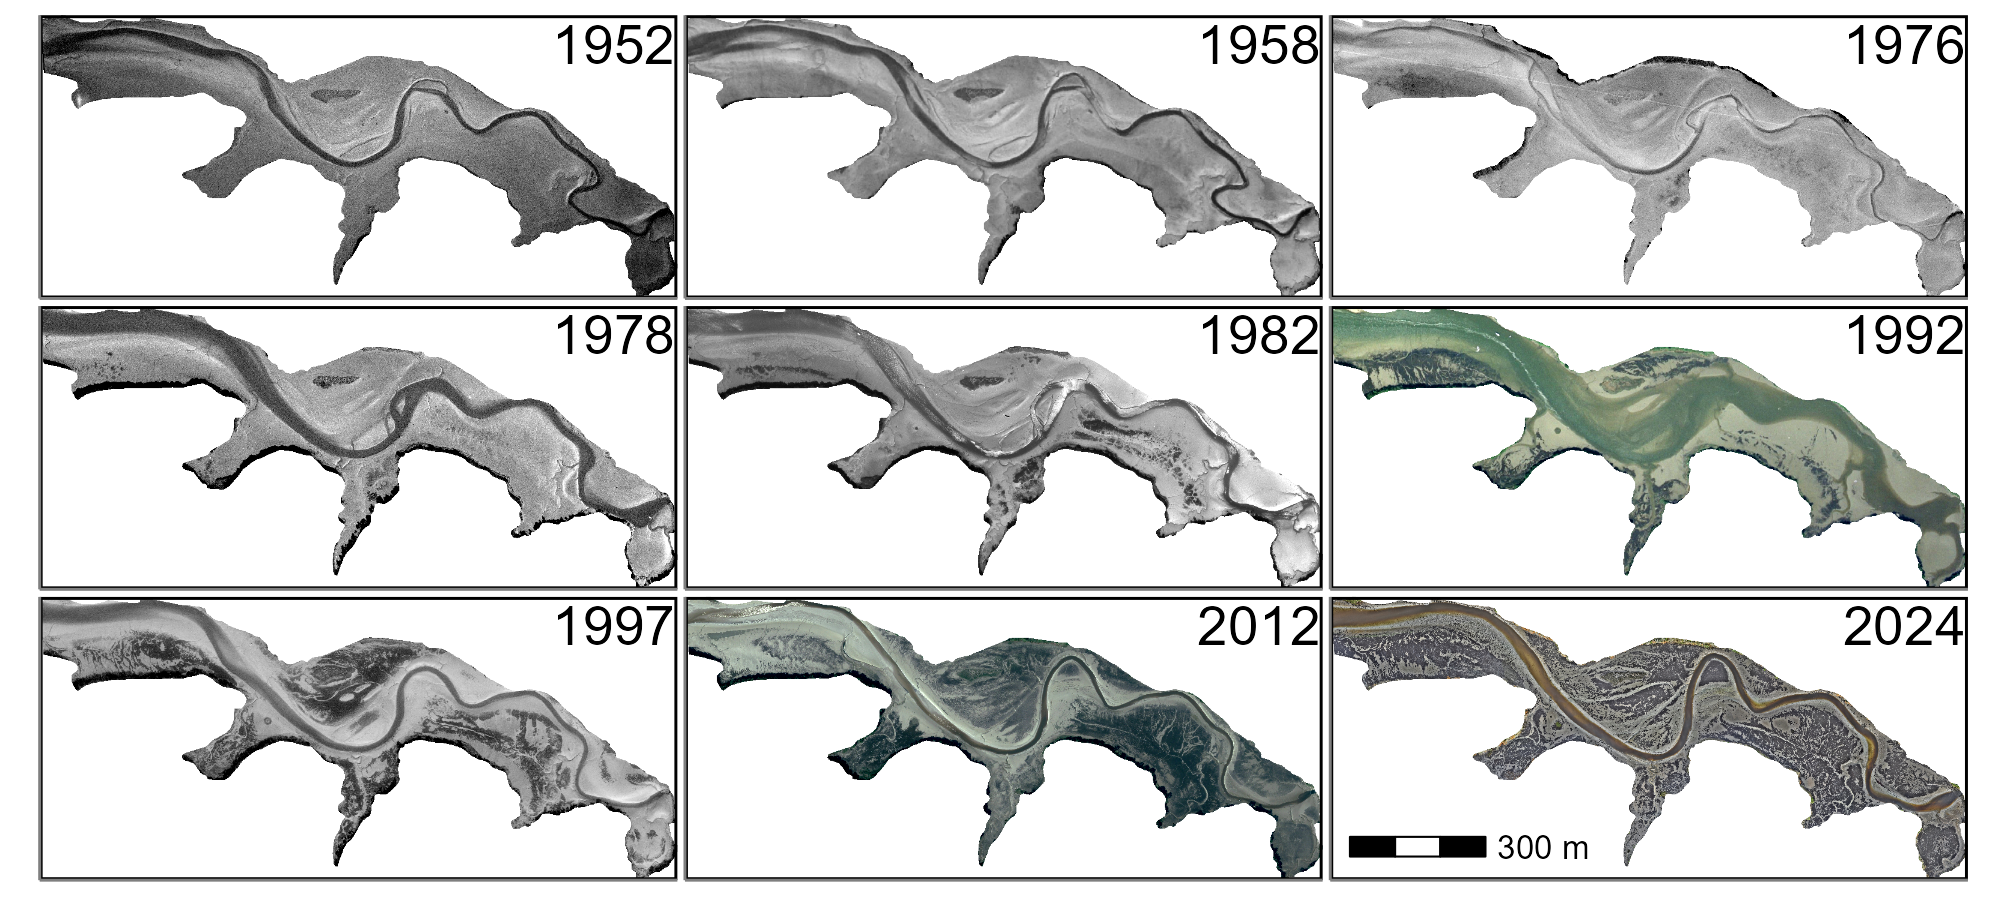
\includegraphics[width=0.95\linewidth,height=\textheight,keepaspectratio]{./Figures/Low_res/Historical_maps.png}

}

\caption{\label{fig-HistoricalMap}Historical images of Pont du Guilly
between 1952 and 2024.}

\end{figure}%

From the early recordings in the 1950s through the late 1970s,
\emph{Gracilaria vermiculophylla} coverage remained effectively at 0\%
(Figure~\ref{fig-HistoricalPlot}). Shortly after the introduction of
\emph{Crassostrea gigas} in the estuary (see vertical red dashed line in
the figure), the first detectable presence of \emph{G. vermiculophylla}
emerged. By 1976, it covered 2.5\% (0.7 ha) of the Pont du Guilly area,
and by 1978 it had increased slightly to 3.0\% (0.9 ha). From 1982
onward, coverage expanded more rapidly, increasing from 6.6\% (2.0 ha)
in 1982 to 14.7\% (4.5 ha) in 1992 and nearly 30\% (9.0 ha) by 1997.
This upward trend continued into the 21st century, peaking at 43.8\%
(13.3 ha) in 2012. Although coverage fluctuated somewhat thereafter
(40.6\% in 2019 and 40.2\% in 2024), it remained consistently high,
indicating sustained and widespread colonization.

\phantomsection\label{cell-fig-HistoricalPlot}
\begin{figure}[H]

\centering{

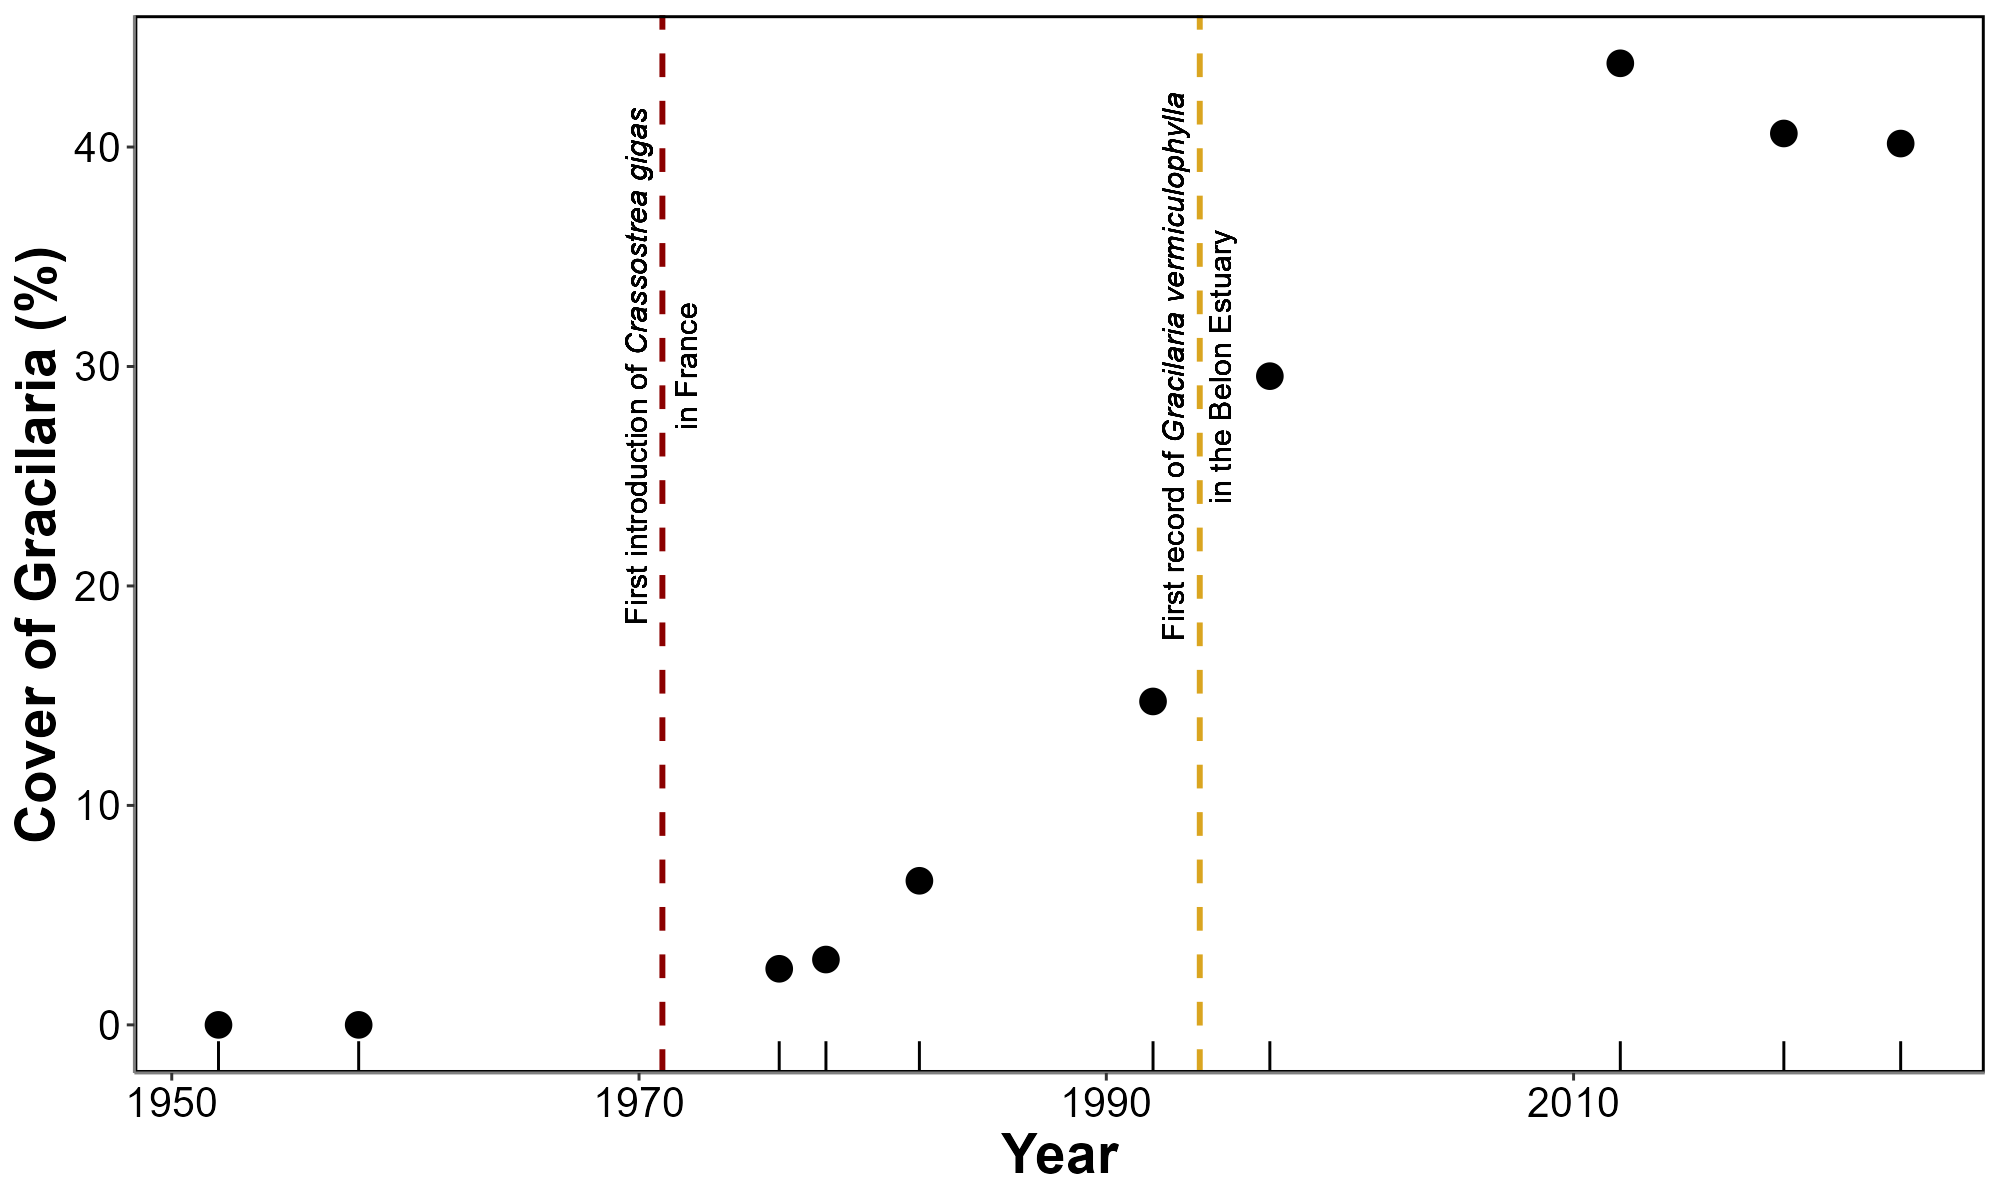
\includegraphics[width=0.95\linewidth,height=\textheight,keepaspectratio]{./Figures/Low_res/Cover_Gracillaria_vs_Time.png}

}

\caption{\label{fig-HistoricalPlot}Evolution of the Gracilaria
vermiculophylla cover at Pont du Guilly in the Belon Estuary. The red
vertical line indicates the date of Crassostrea gigas introduction in
France (Grizel and Heral, 1991), while the golden line represents the
date of the first documented mention of Gracilaria vermiculophylla
invasion in France in the literature (Rueness, 2005).}

\end{figure}%

\subsection{Classification}\label{classification}

The classification map illustrates the diversity of benthic communities
and substrates in the study area (Figure~\ref{fig-Belon} A and B).
Rhodophyceae (red) emerges as the dominant algal cover, forming
extensive, continuous patches aligned with the mid-intertidal zones. In
contrast, Bacillariophyceae (orange) and Chlorophyceae (green) exhibit
more localized distributions, typically restricted to smaller,
fragmented patches where specific microtopographic or hydrodynamic
conditions favor their presence. Phaeophyceae (brown) is confined to
limited patches, often found near transitional zones between sediment
and water or in the upper intertidal area, where it is attached to rocky
substrates. The water class (blue) delineates the main tidal channel,
which meanders through the center of the area and influences the
distribution of adjacent habitats.

The bathymetric map reveals a continuous gradient in elevation relative
to mean sea level (Figure~\ref{fig-Belon} C). A comparison of bathymetry
and vegetation distribution highlights a clear elevation-driven pattern
in algal presence. Higher intertidal zones, located above the deeper
channel areas, are associated with more extensive algal communities. In
contrast, lower intertidal zones closer to the channel consistently
exhibit reduced macroalgal cover.

\phantomsection\label{cell-fig-Belon}
\begin{figure}[H]

\centering{

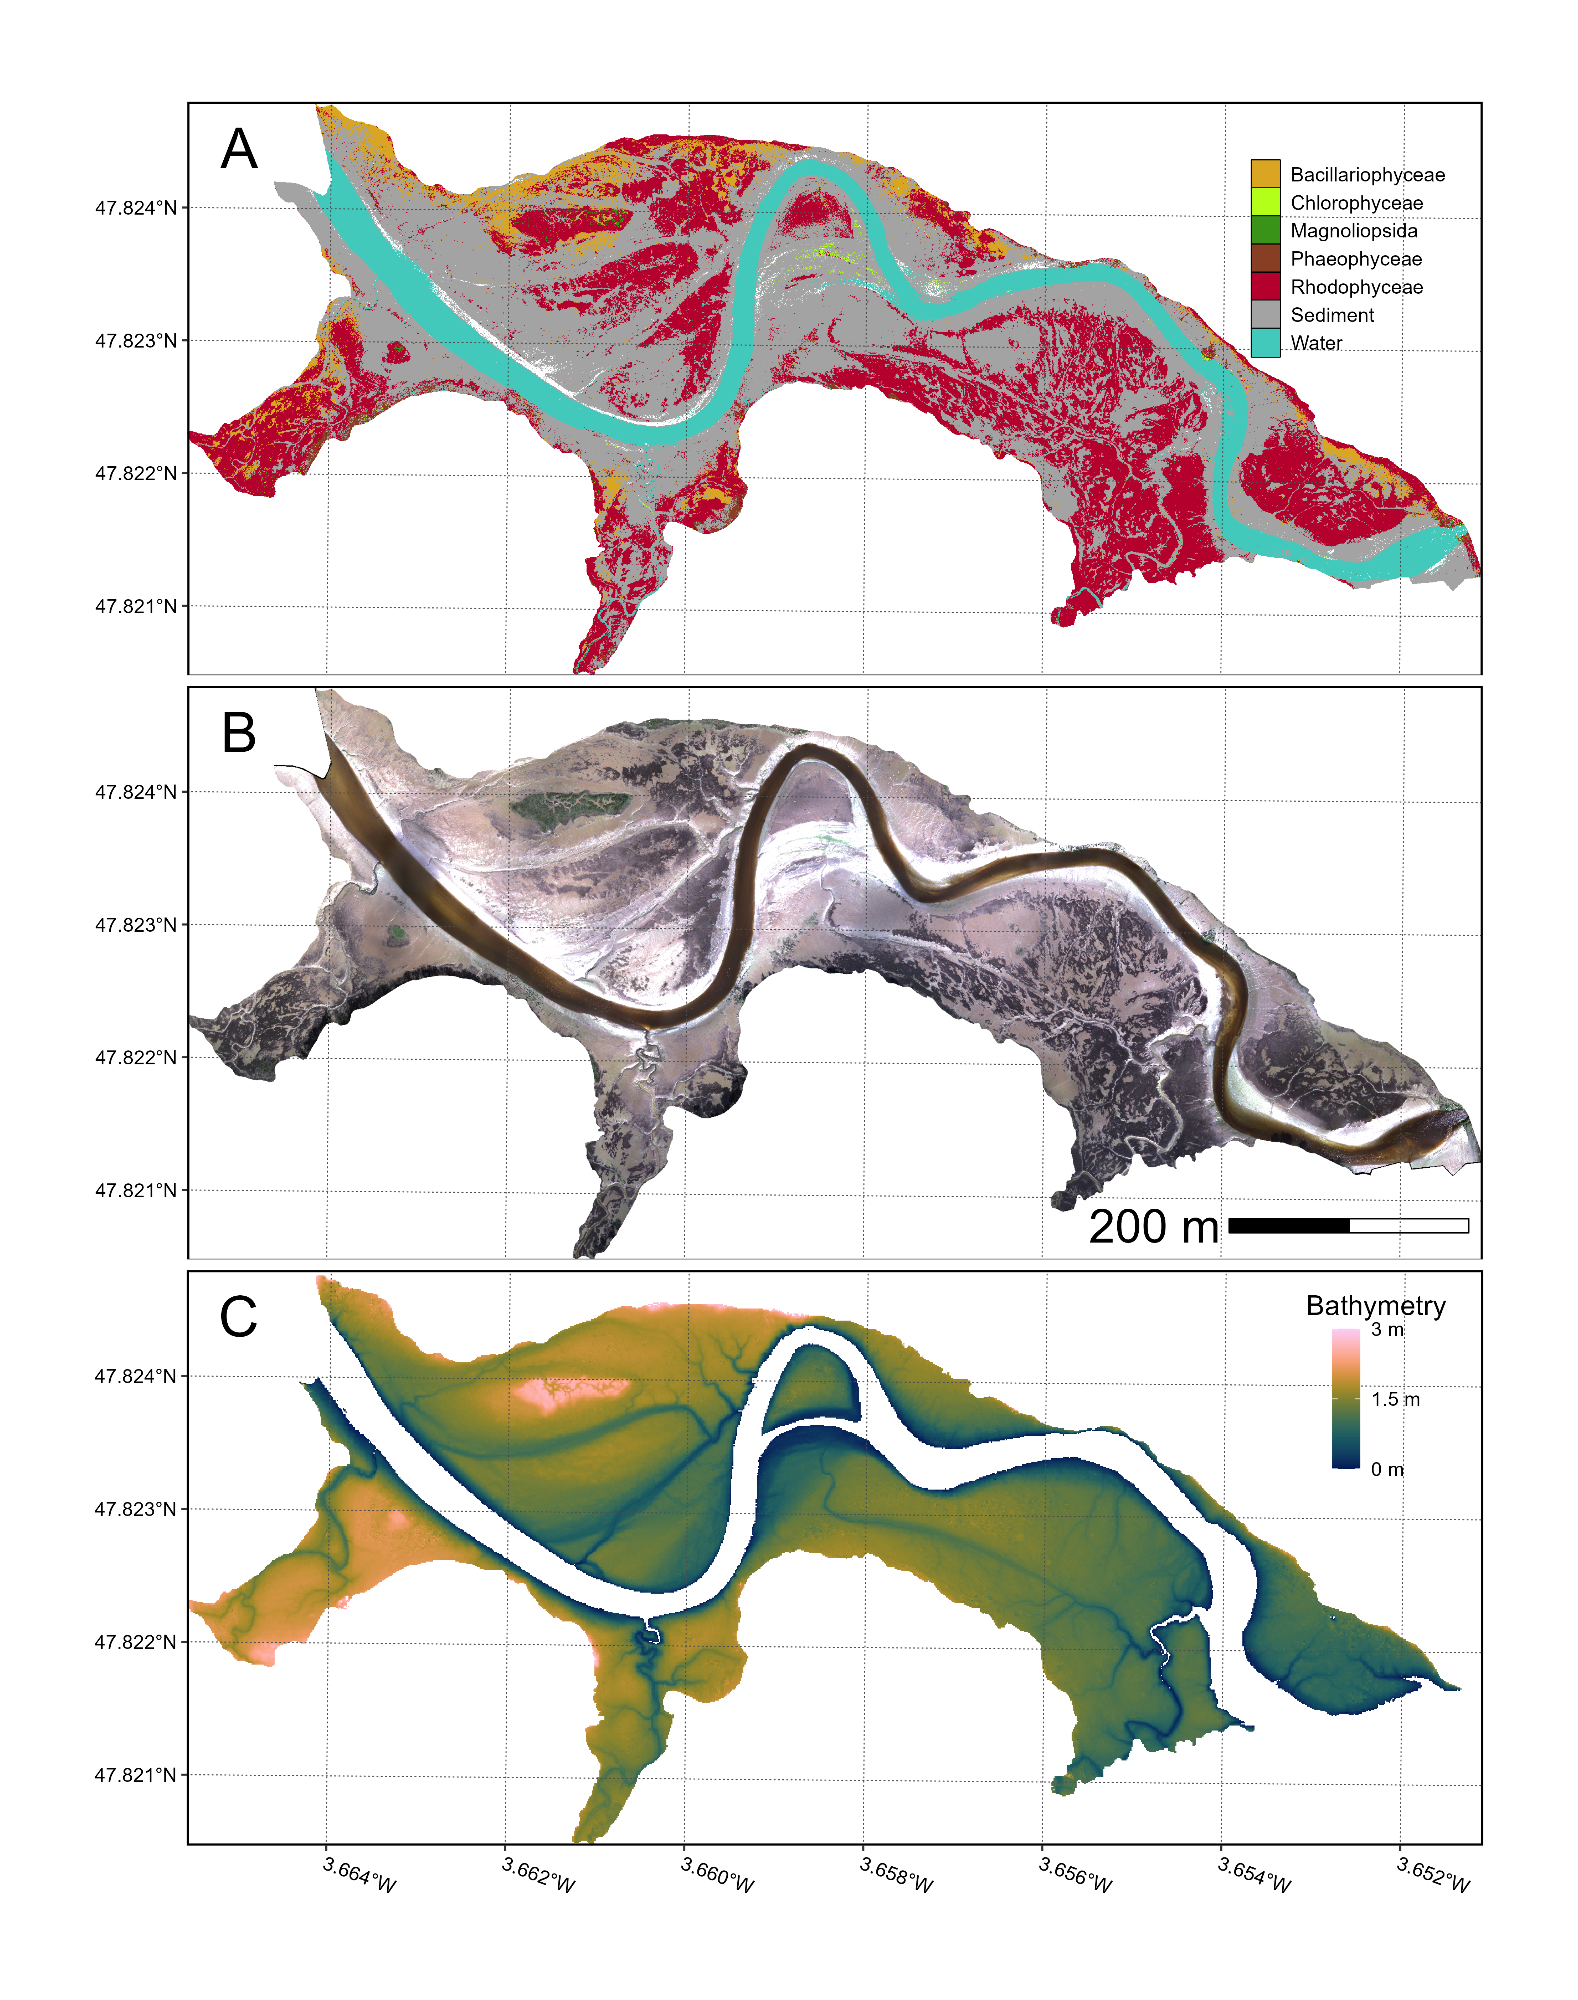
\includegraphics[width=0.95\linewidth,height=\textheight,keepaspectratio]{./Figures/Low_res/Belon_maps.png}

}

\caption{\label{fig-Belon}DISCOV Prediction (A), RGB composition (B) and
Bathymetry (C) of the Bélon estuary site in Brttany, France. The total
extent of this flight was 21 hectars with a resolution of 8 mm per
pixel. Bathymetry is represented as the height above mean sea level.}

\end{figure}%

\subsection{Spectral description}\label{spectral-description}

\subsection{Spatial distribution}\label{spatial-distribution}

\section{Discussion}\label{discussion}

\subsection{\texorpdfstring{Drone mapping \emph{G. vermiculophylla} with
machine
learning}{Drone mapping G. vermiculophylla with machine learning}}\label{drone-mapping-g.-vermiculophylla-with-machine-learning}

In this study, we produced the first spatial distribution maps of the
invasive red alga \emph{Gracilaria vermiculophylla} using a
multispectral drone survey conducted at low tide in Atlantic estuaries
representing varied environmental conditions. In southern Brittany, the
species formed monospecific mats, while in the Cantabrian region of
Spain, it was intermixed with other intertidal vegetation.
Distinguishing among these vegetation types was a key prerequisite for
the analysis.

To achieve this, we adapted the deep learning-based classification model
DISCOV (Oiry et al., 2024b), initially developed to discriminate
seagrass from green macroalgae. Although the original model included
Rhodophyceae as a class, this group constituted less than 3\% of its
training dataset. In contrast, the updated model presented here was
trained on a dataset in which \emph{G. vermiculophylla} covered 26\% of
approximately one million pixels. This improved dataset allowed the
model to achieve an accuracy of \textbf{X\%}.

Rhodophytes possess unique phycobilin pigments, enabling their spectral
distinction from other macroalgal groups (Douay et al., 2022; Mcilwaine
et al., 2019; Olmedo-Masat et al., 2020). Even with the ten-band
multispectral sensor used in our study, it remained feasible to
discriminate the major classes of intertidal macrophytes (Davies et al.,
2023; Oiry et al., 2024b; Román et al., 2021). However, the model
identifies \emph{G. vermiculophylla} at the class level (Rhodophyceae)
rather than at the species level. Although hyperspectral approaches may
allow finer taxonomic resolution (Douay et al., 2022; Olmedo-Masat et
al., 2020), it is unlikely that Gracilaria species can be precisely
distinguished using standard multispectral sensors.

Ecological factors also aid in differentiating \emph{G.
vermiculophylla}. Unlike many other macroalgae that require hard
substrates,* G. vermiculophylla* establishes itself on soft-bottom
sediments. In fact, it is commonly found on mudflats, anchoring its
thalli in the top 10 cm of mud (Surget, 2017), and inhabits the upper
intertidal zone---an unusual trait for a Rhodophyte (Abreu et al., 2011;
Davoult et al., 2017). By reliably detecting \emph{G. vermiculophylla}
in these soft-substrate, upper intertidal habitats, our method provides
a framework for identifying environmental conditions that favor its
spread, potentially offering managers early-warning indicators to
control its expansion before it reaches nuisance levels. Thus, combining
spectral data with sediment characteristics provides a strong indicator
of \emph{G. vermiculophylla} presence in European Atlantic estuaries,
complementing the physical variables already used in species
distribution modeling (Mendoza-Segura et al., 2023).

In addition, the scalability of drone-based surveying facilitates repeat
mapping to detect temporal shifts in the distribution and abundance of
\emph{G. vermiculophylla.} Such continuous monitoring could capture
seasonal patterns of colonization, allowing researchers and
environmental managers to evaluate the effectiveness of mitigation
measures, track long-term ecological impacts, and anticipate future
shifts in habitat suitability under changing climate conditions.

\subsection{\texorpdfstring{\emph{G. vermiculophylla} spatial
distribution and mudflat
topography}{G. vermiculophylla spatial distribution and mudflat topography}}\label{g.-vermiculophylla-spatial-distribution-and-mudflat-topography}

\subsection{Spatio-temporal monitoring of invasive
macroalgae}\label{spatio-temporal-monitoring-of-invasive-macroalgae}

Accurate, high-resolution maps of invasive or alien species are
extremely scarce (\textbf{REF}), yet they enable in-depth evaluations of
these species' ecology, temporal dynamics, and niche behavior in
relation to their environment. In this study, using individual flights
over monospecific algal mats, we quantified how this invasive alga
associates with local mudflat topography, demonstrating that
\textbf{\ldots{}}. Repeated monitoring of this type can further reveal
phenological patterns, invasion dynamics, and local conspecific
biological interactions---such as co-occurrence, displacement, or
avoidance (\textbf{REF}).

Remote sensing using multispectral drone mapping can provide
high-resolution, spatially explicit data, but it must be combined with
repeated, in situ field measurements to maximize its potential
(\textbf{REF}). As noted, temporal repetition makes it possible to
assess dynamic processes, and integrating these mapping approaches with
in situ analyses of local infauna, carbon cycling, riverine inputs, and
sedimentology would yield valuable insights for local managers. Such an
integrated approach could help determine how the invasive alga affects
the local ecosystem and, more broadly, forecast its potential impact on
other estuarine environments facing similar invasion events. This
holistic approach can guide strategic interventions aimed at mitigating
the alga's spread, maintaining ecological balance, and protecting native
biodiversity, ensuring that management efforts are informed by accurate,
timely, and spatially explicit data.

Invasive species like \emph{Gracilaria vermiculophylla} and
\emph{Rugulopteryx okamurae} can be identified using drones equipped
with multispectral sensors, taking advantage of the characteristic
reflectance of rhodophytes (Roca et al., 2022). However, this capability
has not yet been tested using standard RGB sensors found in readily
available commercial drones. These drones are easy to deploy, can cover
large areas when flying at speeds of 15 m s\^{}-1 at an altitude of 120
m, and still maintain sufficient overlap between images to support
photogrammetric reconstruction. Expanding these methodologies to
RGB-based detection would significantly lower barriers to entry,
allowing local stakeholders with limited resources to access valuable
monitoring tools for early detection and rapid response. A promising
avenue for operational applications lies in testing machine learning
techniques on RGB imagery that do not rely on enhanced spectral
resolution. Considering the low cost of RGB and multispectral commercial
drones, coupled with ongoing advancements in machine learning,
drone-based remote sensing has now matured into a practical tool for
adoption by environmental authorities in coastal management. Integrating
these technologies into routine monitoring protocols can enhance
surveillance capabilities, improve understanding of invasive species
dynamics, and ultimately contribute to more effective conservation and
restoration strategies.

\section{Conclusion}\label{conclusion}

\section*{References}\label{references}
\addcontentsline{toc}{section}{References}

\phantomsection\label{refs}
\begin{CSLReferences}{1}{0}
\bibitem[\citeproctext]{ref-abreu2011nitrogen}
Abreu, M.H., Pereira, R., Buschmann, A., Sousa-Pinto, I., Yarish, C.,
2011. Nitrogen uptake responses of gracilaria vermiculophylla (ohmi)
papenfuss under combined and single addition of nitrate and ammonium.
Journal of Experimental Marine Biology and Ecology 407, 190--199.

\bibitem[\citeproctext]{ref-agisoft}
Agisoft, 2019. \href{https://www.agisoft.com/}{Agisoft metashape}.

\bibitem[\citeproctext]{ref-Blanchet2014}
Blanchet, H., Gouillieux, B., Alizier, S., others, 2014. Multiscale
patterns in the diversity and organization of benthic intertidal fauna
among french atlantic estuaries. Journal of Sea Research 90, 95--110.
\url{https://doi.org/10.1016/j.seares.2014.02.014}

\bibitem[\citeproctext]{ref-brunier2022evolution}
Brunier, G., Tamura, T., Anthony, E.J., Dussouillez, P., Gardel, A.,
2022. Evolution of the french guiana coast from late pleistocene to
holocene based on chenier and beach sand dating. Regional Environmental
Change 22, 122.

\bibitem[\citeproctext]{ref-calleja2017long}
Calleja, F., Galván, C., Silió-Calzada, A., Juanes, J.A., Ondiviela, B.,
2017. Long-term analysis of zostera noltei: A retrospective approach for
understanding seagrasses' dynamics. Marine environmental research 130,
93--105.

\bibitem[\citeproctext]{ref-Castaing1995}
Castaing, P., Guilcher, A., 1995. Morphosedimentary evolution of
ria-type estuaries. Earth Surface Processes and Landforms 20, 361--376.
\url{https://doi.org/10.1002/esp.3290200408}

\bibitem[\citeproctext]{ref-chand2021low}
Chand, S., Bollard, B., 2021. Low altitude spatial assessment and
monitoring of intertidal seagrass meadows beyond the visible spectrum
using a remotely piloted aircraft system. Estuarine, Coastal and Shelf
Science 255, 107299.

\bibitem[\citeproctext]{ref-davies2023multi}
Davies, B.F.R., Gernez, P., Geraud, A., Oiry, S., Rosa, P., Zoffoli,
M.L., Barillé, L., 2023. Multi-and hyperspectral classification of
soft-bottom intertidal vegetation using a spectral library for coastal
biodiversity remote sensing. Remote Sensing of Environment 290, 113554.

\bibitem[\citeproctext]{ref-davies2024sentinel}
Davies, B.F.R., Oiry, S., Rosa, P., Zoffoli, M.L., Sousa, A.I., Thomas,
O.R., Smale, D.A., Austen, M.C., Biermann, L., Attrill, M.J., others,
2024b. A sentinel watching over inter-tidal seagrass phenology across
western europe and north africa. Communications Earth \& Environment 5,
382.

\bibitem[\citeproctext]{ref-davies2024intertidal}
Davies, B.F.R., Oiry, S., Rosa, P., Zoffoli, M.L., Sousa, A.I., Thomas,
O.R., Smale, D.A., Austen, M.C., Biermann, L., Attrill, M.J., others,
2024a. Intertidal seagrass extent from sentinel-2 time-series show
distinct trajectories in western europe. Remote Sensing of Environment
312, 114340.

\bibitem[\citeproctext]{ref-davoult2017multiple}
Davoult, D., Surget, G., Stiger-Pouvreau, V., Noisette, F., Riera, P.,
Stagnol, D., Androuin, T., Poupart, N., 2017. Multiple effects of a
gracilaria vermiculophylla invasion on estuarine mudflat functioning and
diversity. Marine Environmental Research 131, 227--235.

\bibitem[\citeproctext]{ref-rs14133124}
Diruit, W., Le Bris, A., Bajjouk, T., Richier, S., Helias, M., Burel,
T., Lennon, M., Guyot, A., Ar Gall, E., 2022. Seaweed habitats on the
shore: Characterization through hyperspectral UAV imagery and field
sampling. Remote Sensing 14. \url{https://doi.org/10.3390/rs14133124}

\bibitem[\citeproctext]{ref-rs14020346}
Douay, F., Verpoorter, C., Duong, G., Spilmont, N., Gevaert, F., 2022.
New hyperspectral procedure to discriminate intertidal macroalgae.
Remote Sensing 14. \url{https://doi.org/10.3390/rs14020346}

\bibitem[\citeproctext]{ref-douglas2024linking}
Douglas, T.J., Coops, N.C., Drever, M.C., Hunt, B.P., Martin, T.G.,
2024. Linking microphytobenthos distribution and mudflat geomorphology
under varying sedimentary regimes using unoccupied aerial vehicle
(UAV)-acquired multispectral reflectance and photogrammetry. Science of
The Total Environment 173675.

\bibitem[\citeproctext]{ref-duffy2018spatial}
Duffy, J.P., Pratt, L., Anderson, K., Land, P.E., Shutler, J.D., 2018.
Spatial assessment of intertidal seagrass meadows using optical imaging
systems and a lightweight drone. Estuarine, Coastal and Shelf Science
200, 169--180.

\bibitem[\citeproctext]{ref-firth2024invasive}
Firth, L.B., Foggo, A., Watts, T., Knights, A.M., DeAmicis, S., 2024.
Invasive macroalgae in native seagrass beds: Vectors of spread and
impacts. Annals of Botany 133, 41--50.

\bibitem[\citeproctext]{ref-van2018global}
Ginneken, V. van, Vries, E. de, others, 2018. The global dispersal of
the non-endemic invasive red alga gracilaria vermiculophylla in the
ecosystems of the euro-asia coastal waters including the wadden sea
unesco world heritage coastal area: Awful or awesome? Oceanography \&
Fisheries Open Access Journal 8, 4--26.

\bibitem[\citeproctext]{ref-grizel1991introduction}
Grizel, H., Heral, M., 1991. Introduction into france of the japanese
oyster (crassostrea gigas). ICES Journal of Marine Science 47, 399--403.

\bibitem[\citeproctext]{ref-gurgel2018systematics}
Gurgel, C.F.D., Norris, J.N., Schmidt, W.E., Le, H.N., Fredericq, S.,
2018. Systematics of the gracilariales (rhodophyta) including new
subfamilies, tribes, subgenera, and two new genera, agarophyton gen.
Nov. And crassa gen. nov. Phytotaxa 374, 1--23.

\bibitem[\citeproctext]{ref-krueger2017genetic}
Krueger-Hadfield, S.A., Kollars, N.M., Strand, A.E., Byers, J.E.,
Shainker, S.J., Terada, R., Greig, T.W., Hammann, M., Murray, D.C.,
Weinberger, F., others, 2017. Genetic identification of source and
likely vector of a widespread marine invader. Ecology and evolution 7,
4432--4447.

\bibitem[\citeproctext]{ref-d15020161}
Massé, C., Viard, F., Humbert, S., Antajan, E., Auby, I., Bachelet, G.,
Bernard, G., Bouchet, V.M.P., Burel, T., Dauvin, J.-C., Delegrange, A.,
Derrien-Courtel, S., Droual, G., Gouillieux, B., Goulletquer, P.,
Guérin, L., Janson, A.-L., Jourde, J., Labrune, C., Lavesque, N.,
Leclerc, J.-C., Le Duff, M., Le Garrec, V., Noël, P., Nowaczyk, A.,
Pergent-Martini, C., Pezy, J.-P., Raoux, A., Raybaud, V., Ruitton, S.,
Sauriau, P.-G., Spilmont, N., Thibault, D., Vincent, D., Curd, A., 2023.
An overview of marine non-indigenous species found in three contrasting
biogeographic metropolitan french regions: Insights on distribution,
origins and pathways of introduction. Diversity 15.
\url{https://doi.org/10.3390/d15020161}

\bibitem[\citeproctext]{ref-rs11060704}
Mcilwaine, B., Casado, M.R., Leinster, P., 2019. Using 1st derivative
reflectance signatures within a remote sensing framework to identify
macroalgae in marine environments. Remote Sensing 11.
\url{https://doi.org/10.3390/rs11060704}

\bibitem[\citeproctext]{ref-jmse11020367}
Mendoza-Segura, C., Fernández, E., Beca-Carretero, P., 2023. Predicted
changes in the biogeographical range of gracilaria vermiculophylla under
present and future climate scenarios. Journal of Marine Science and
Engineering 11. \url{https://doi.org/10.3390/jmse11020367}

\bibitem[\citeproctext]{ref-Michel2021}
Michel, G., Le Bot, S., Lesourd, S., Lafite, R., 2021.
Morpho-sedimentological and dynamic patterns in a ria type estuary: The
belon estuary (south brittany, france). Journal of Maps 17, 389--400.
\url{https://doi.org/10.1080/17445647.2021.1925170}

\bibitem[\citeproctext]{ref-nebel2020review}
Nebel, S., Beege, M., Schneider, S., Rey, G.D., 2020. A review of
photogrammetry and photorealistic 3D models in education from a
psychological perspective, in: Frontiers in Education. Frontiers Media
SA, p. 144.

\bibitem[\citeproctext]{ref-nyberg2007introduced}
Nyberg, C.D., 2007. Introduced marine macroalgae and habitat modifiers:
Their ecological role and significant attributes. Department of Marine
Ecology.

\bibitem[\citeproctext]{ref-nyberg2009flora}
Nyberg, C.D., Thomsen, M.S., Wallentinus, I., 2009. Flora and fauna
associated with the introduced red alga gracilaria vermiculophylla.
European Journal of Phycology 44, 395--403.

\bibitem[\citeproctext]{ref-ohmi1956contributions}
OHMI, H., 1956. CONTRIBUTIONS TO THE KNOWLEDGE OF GRACILARIACEAE FROM
JAPAN: Ⅱ. On a new species of the genus gracilariopsis, with some
considerations on its ecology. 北海道大學水産學部研究彙報 6, 271--279.

\bibitem[\citeproctext]{ref-oiry_2024_14218984}
Oiry, S., Davies, B.F.R., Pierre, G., Laurent, B., 2024a. {DISCOV: Drone
Intertidal Sediment Classification Of Vegetation}.
\url{https://doi.org/10.5281/zenodo.14218984}

\bibitem[\citeproctext]{ref-rs16234383}
Oiry, S., Davies, B.F.R., Sousa, A.I., Rosa, P., Zoffoli, M.L., Brunier,
G., Gernez, P., Barillé, L., 2024b. Discriminating seagrasses from green
macroalgae in european intertidal areas using high-resolution
multispectral drone imagery. Remote Sensing 16.
\url{https://doi.org/10.3390/rs16234383}

\bibitem[\citeproctext]{ref-olmedo2020far}
Olmedo-Masat, O.M., Raffo, M.P., Rodrı́guez-Pérez, D., Arijón, M.,
Sánchez-Carnero, N., 2020. How far can we classify macroalgae remotely?
An example using a new spectral library of species from the south west
atlantic (argentine patagonia). Remote Sensing 12, 3870.

\bibitem[\citeproctext]{ref-ortega2005fluxes}
Ortega, T., Ponce, R., Forja, J., Gómez-Parra, A., 2005. Fluxes of
dissolved inorganic carbon in three estuarine systems of the cantabrian
sea (north of spain). Journal of Marine Systems 53, 125--142.

\bibitem[\citeproctext]{ref-WoRMS303450}
Papenfuss, G.F., 1967.
\href{https://marinespecies.org/aphia.php?p=sourcedetails&id=303450}{Notes
on algal nomenclature - v. Various chlorophyceae and rhodophyceae}.
Phykos 5, 95--105.

\bibitem[\citeproctext]{ref-peidro2024quantifying}
Peidro-Devesa, M.J., Martı́nez-Movilla, A., Rodrı́guez-Somoza, J.L.,
Sánchez, J.M., Román, M., 2024. Quantifying intertidal macroalgae stocks
in the NW iberian peninsula using unmanned aerial vehicle (UAV)
multispectral imagery. Regional Studies in Marine Science 103621.

\bibitem[\citeproctext]{ref-ramus2017invasive}
Ramus, A.P., Silliman, B.R., Thomsen, M.S., Long, Z.T., 2017. An
invasive foundation species enhances multifunctionality in a coastal
ecosystem. Proceedings of the national academy of sciences 114,
8580--8585.

\bibitem[\citeproctext]{ref-roca2022monitoring}
Roca, M., Dunbar, M.B., Román, A., Caballero, I., Zoffoli, M.L., Gernez,
P., Navarro, G., 2022. Monitoring the marine invasive alien species
rugulopteryx okamurae using unmanned aerial vehicles and satellites.
Frontiers in Marine Science 9, 1004012.

\bibitem[\citeproctext]{ref-roman2024mapping}
Román, A., Oiry, S., Davies, B.F., Rosa, P., Gernez, P., Tovar-Sánchez,
A., Navarro, G., Méléder, V., Barillé, L., 2024. Mapping intertidal
microphytobenthic biomass with very high-resolution remote sensing
imagery in an estuarine system. Science of The Total Environment 177025.

\bibitem[\citeproctext]{ref-roman2021using}
Román, A., Tovar-Sánchez, A., Olivé, I., Navarro, G., 2021. Using a
UAV-mounted multispectral camera for the monitoring of marine
macrophytes. Frontiers in Marine Science 8, 722698.

\bibitem[\citeproctext]{ref-romero2008sintering}
Romero, M., Andrés, A., Alonso, R., Viguri, J., Rincón, J.M., 2008.
Sintering behaviour of ceramic bodies from contaminated marine
sediments. Ceramics International 34, 1917--1924.

\bibitem[\citeproctext]{ref-rueness2005life}
Rueness, J., 2005. Life history and molecular sequences of gracilaria
vermiculophylla (gracilariales, rhodophyta), a new introduction to
european waters. Phycologia 44, 120--128.

\bibitem[\citeproctext]{ref-sfriso2012spreading}
Sfriso, A., Wolf, M.A., Maistro, S., Sciuto, K., Moro, I., 2012.
Spreading and autoecology of the invasive species gracilaria
vermiculophylla (gracilariales, rhodophyta) in the lagoons of the
north-western adriatic sea (mediterranean sea, italy). Estuarine,
Coastal and Shelf Science 114, 192--198.

\bibitem[\citeproctext]{ref-sotka2018combining}
Sotka, E.E., Baumgardner, A.W., Bippus, P.M., Destombe, C., Duermit,
E.A., Endo, H., Flanagan, B.A., Kamiya, M., Lees, L.E., Murren, C.J.,
others, 2018. Combining niche shift and population genetic analyses
predicts rapid phenotypic evolution during invasion. Evolutionary
Applications 11, 781--793.

\bibitem[\citeproctext]{ref-surget2017processus}
Surget, G., 2017. Processus adaptatifs des v{é}g{é}taux marins face au
changement climatique {à} diff{é}rentes {é}chelles de temps et d'espace:
Dynamique de populations, m{é}tabolomique, {é}cophysiologie et
potentiels de valorisation (PhD thesis). Universit{é} de Bretagne
occidentale-Brest.

\bibitem[\citeproctext]{ref-Tankoua2011}
Tankoua, O.F., Buffet, P.-E., Amiard, J.-C., Amiard-Triquet, C.,
Mouneyrac, C., Berthet, B., 2011. Potential influence of confounding
factors (size, salinity) on biomarkers in the sentinel species
scrobicularia plana used in programmes monitoring estuarine quality.
Environmental Science and Pollution Research 18, 1253--1263.
\url{https://doi.org/10.1007/s11356-011-0479-3}

\bibitem[\citeproctext]{ref-terada2002review}
Terada, R., Yamamoto, H., 2002. Review of gracilaria vermiculophylla
(ohmi) papenfuss and other species in japan and asia. Taxonomy of
economic seaweeds, with special reference to Pacific species 8,
225--230.

\bibitem[\citeproctext]{ref-thomsen2007gracilaria}
Thomsen, M.S., Staehr, P.A., Nyberg, C.D., Schwærter, S., Krause-Jensen,
D., Silliman, B.R., 2007. Gracilaria vermiculophylla (ohmi) papenfuss,
1967 (rhodophyta, gracilariaceae) in northern europe, with emphasis on
danish conditions, and what to expect in the future. Aquatic invasions
2, 83--94.

\bibitem[\citeproctext]{ref-thomsen2013effects}
Thomsen, M.S., Stæhr, P.A., Nejrup, L., Schiel, D.R., 2013. Effects of
the invasive macroalgae gracilaria vermiculophylla on two co-occurring
foundation species and associated invertebrates. Aquatic Invasions 8,
133--145.

\bibitem[\citeproctext]{ref-valle2015mapping}
Valle, M., Pala, V., Lafon, V., Dehouck, A., Garmendia, J.M., Borja, A.,
Chust, G., 2015. Mapping estuarine habitats using airborne hyperspectral
imagery, with special focus on seagrass meadows. Estuarine, Coastal and
Shelf Science 164, 433--442.

\bibitem[\citeproctext]{ref-van2003reintroduction}
Van Katwijk, M., 2003. Reintroduction of eelgrass (zostera marina l.) in
the dutch wadden sea: A research overview and management vision, in:
Challenges to the Wadden Sea Area. In: Proceedings of the 10th
International Scientific Wadden Sea Symposium, Groningen, the
Netherlands. pp. 173--195.

\bibitem[\citeproctext]{ref-weinberger2008invasive}
Weinberger, F., Buchholz, B., Karez, R., Wahl, M., 2008. The invasive
red alga gracilaria vermiculophylla in the baltic sea: Adaptation to
brackish water may compensate for light limitation. Aquatic Biology 3,
251--264.

\bibitem[\citeproctext]{ref-williams2007global}
Williams, S.L., Smith, J.E., 2007. A global review of the distribution,
taxonomy, and impacts of introduced seaweeds. Annu. Rev. Ecol. Evol.
Syst. 38, 327--359.

\bibitem[\citeproctext]{ref-d14121077}
Zenetos, A., Tsiamis, K., Galanidi, M., Carvalho, N., Bartilotti, C.,
Canning-Clode, J., Castriota, L., Chainho, P., Comas-González, R.,
Costa, A.C., Dragičević, B., Dulčić, J., Faasse, M., Florin, A.-B.,
Gittenberger, A., Jakobsen, H., Jelmert, A., Kerckhof, F., Lehtiniemi,
M., Livi, S., Lundgreen, K., Macic, V., Massé, C., Mavrič, B., Naddafi,
R., Orlando-Bonaca, M., Petovic, S., Png-Gonzalez, L., Carbonell
Quetglas, A., Ribeiro, R.S., Cidade, T., Smolders, S., Stæhr, P.A.U.,
Viard, F., Outinen, O., 2022. Status and trends in the rate of
introduction of marine non-indigenous species in european seas.
Diversity 14. \url{https://doi.org/10.3390/d14121077}

\bibitem[\citeproctext]{ref-zoffoli2021decadal}
Zoffoli, M.L., Gernez, P., Godet, L., Peters, S., Oiry, S., Barillé, L.,
2021. Decadal increase in the ecological status of a north-atlantic
intertidal seagrass meadow observed with multi-mission satellite
time-series. Ecological Indicators 130, 108033.

\end{CSLReferences}




\end{document}
